%BEGIN: SIMACT
\section{SIMACT: a 3D Open Source Smart Home Simulator for Activity Recognition with Open Database and Visual Editor}\label{sec:simact}

SIMACT is a flexible 3D smart home infrastructure simulator, developed in Java, specifically designed to help researchers working in the field of activity recognition \cite{bouchard2012simact}. The simulator is released as open-source \cite{bouchard:simact:Online} under GPLv3 \cite{gpl:v3}.\\

This work is specifically focused on the interaction between an agent and the surrounding environment in the smart house. It is built to reproduce everyday life scenarios, on a step-by-step basis. Entire scenarios and interactions can be designed only by writing using scripts and visual editors, without having to write one line of code.\\

The simulator is built entailer on Java based technologies. The GUI is based on the swing library, while the 3D renderer is based on the Java Monkey Engine\footnote{\url{http://jmonkeyengine.org/}}. For the 3D design, they have used a modeling tool for house design and interior accessories from Google called SketchUp \cite{sketchup:online}. This comes with a great advantage as SketchUp's community maintains a huge library of free 3D models, where one can find almost any accessory that would fit in a home.\\

To further detail, I will briefly discuss the on the system's architecture, as illustrated in Figure \ref{fig:simact_architecture}.

\begin{figure}[H]
	\centering
	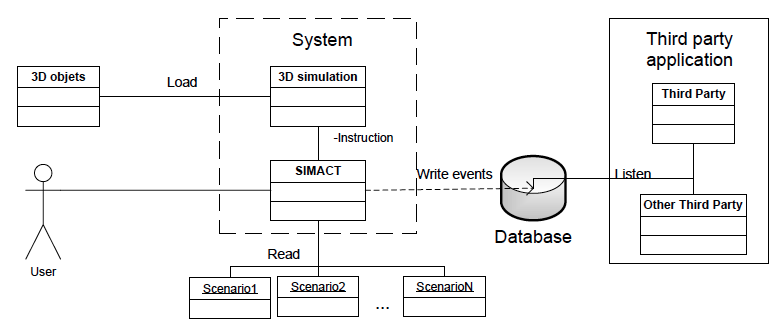
\includegraphics[width=\linewidth]{gfx/Chapter2/simact_architecture}
	\caption{SIMACT: System Architecture}
	\label{fig:simact_architecture}
\end{figure}

To create a custom simulation, a researcher starts out by defining the environment, by defining the object models contained within. The simulator loads these definitions to create the virtual model of the environment and to initialize the 3D simulator. To define the interaction with the habitat, the researcher provides the simulator with an XML file defining the interaction scenario. The scenario is defined as a sequence of steps, which is read, interpreted and execute by the simulator (it plays the role of an interpreter). As the steps are executed and the environment gets modified by these actions, the generated events are written into a database. Further, third party applications can communicate with the database to retrieve data in real-time, which can be used in the logic of the application.\\

A snapshot of the simulation tool in action is depicted in Figure \ref{fig:simact_simulation_tool}.

\begin{figure}[H]
	\centering
	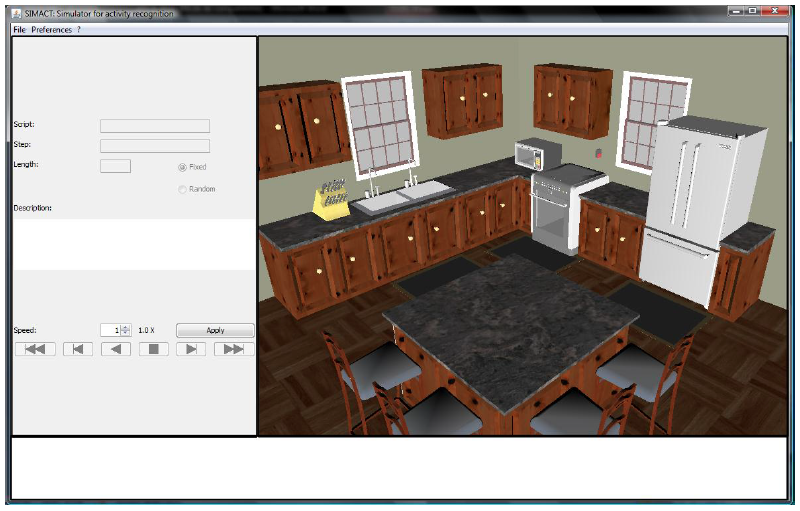
\includegraphics[width=\linewidth]{gfx/Chapter2/simact_simulation_tool}
	\caption{SIMACT: Simulation Tool in Action}
	\label{fig:simact_simulation_tool}
\end{figure}

This tool provides a powerful and reusable simulation environment, with a strong platform worth considering as basis for the simulator I am targeting to develop. My only concern is that I have not been able to determine the complexity of adding support for device simulation, as the main target of SIMACT is interaction with the physical environment.\\

In conclusion, I will allocate some time during the system design process to analyze in detail if building on top of SIMACT would be possible.
%END: SIMACT